
\documentclass[12pt,a4paper]{article}

\usepackage{allrunes}
\usepackage{amsmath}
\usepackage[magyar]{babel}
\usepackage[T1]{fontenc}
\usepackage[utf8]{inputenc}
\usepackage{fixltx2e}
\usepackage{multirow}
\usepackage{hyperref}
\usepackage{amsfonts}
\usepackage{amsthm}
\usepackage{amssymb}
\usepackage{indentfirst}

\usepackage[a4paper]{geometry}

\geometry{a4paper,
		     tmargin = 35mm, 
		     lmargin = 25mm,
		     rmargin = 30mm,
		     bmargin = 30mm}

\theoremstyle{plain}
\usepackage{graphicx}

\usepackage{float}
\renewcommand\thesection{\Roman{section}}

\title{\textbf{Folyadékszcintillációs spektroszkópia}}

\author{\Large{\textsc{Olar Alex}} \vspace{10pt}\\
	\textrm{Eötvös Loránd Tudományegyetem}
	}
\date{}
%\lhead{}
\begin{document}
\addtolength{\voffset}{-1.0cm}
\addtolength{\textheight}{1.0cm}
\begin{titlepage}
	\maketitle

	\vfill

	\begin{figure}[H]
		\centering
		
\includegraphics[scale=0.6]{eltecimer.jpg}
	\end{figure}

	\thispagestyle{empty}
\end{titlepage}

\section{Mérés célja}
\hspace*{10pt} A labor során megismerkedtünk
a folyadékszcintillációs spektroszkópia módszerével.

\section{Elméleti összefoglaló}
\hspace*{10pt} A mérés során a negatív béta-bomló trícium atomot
vizsgáltuk és ennek kaptuk meg 19 db spektrumát. A bomló trícium
a bomlás során kibocsájt egy elektront és héliummá alakul, az
elektronokat koincidenciában lehetőségünk van detektálni egy fotoelektron
sokszorozó segítségével.

\vspace{0.2cm}

\par A felszabaduló energia nem kizárólag az elektronra fordítódik, hiszen egy
antineutrínó is keletkezik a folyamat során így az elektron energia spektruma
folytonos lesz. Az alakja jellemezhető a következő formulával.

\vspace{0.2cm}

\begin{equation}
	\rho (E) dE \sim \sqrt{E}(Q-E)^2
\end{equation}

\vspace{0.2cm}

A kapott kifejezéssel felírva a várható értéket:

\vspace{0.2cm}

\begin{equation}
	\big<E\big> = \frac{1}{3}Q
\end{equation}

\vspace{0.2cm}

\par A bomlás során maximálisan 18.6 keV energia szabadul fel,
ennek harmada az mely a várható érték lesz.

\vspace{0.2cm}

\begin{equation}
	\big<E\big>\approx 6.2 \textrm{ keV}
\end{equation}

\vspace{0.2cm}

\par A kiértékelés során megillesztettük az (1)-es összefüggést, majd
kiszámoltuk az energia várható értékét a súlyozott átlagokból, majd az
(1)-es összefüggést kiegészítettük a labor mellé kapott cikkből származtatott
Fermi-függvénnyel.

\newpage

\section{Kiértékelés}

\subsection{Átlag spektrum}

\hspace*{10pt} A mért adatok átlag spektruma hibákkal:

\vspace{0.2cm}

\begin{figure}[!h]
	\centering
	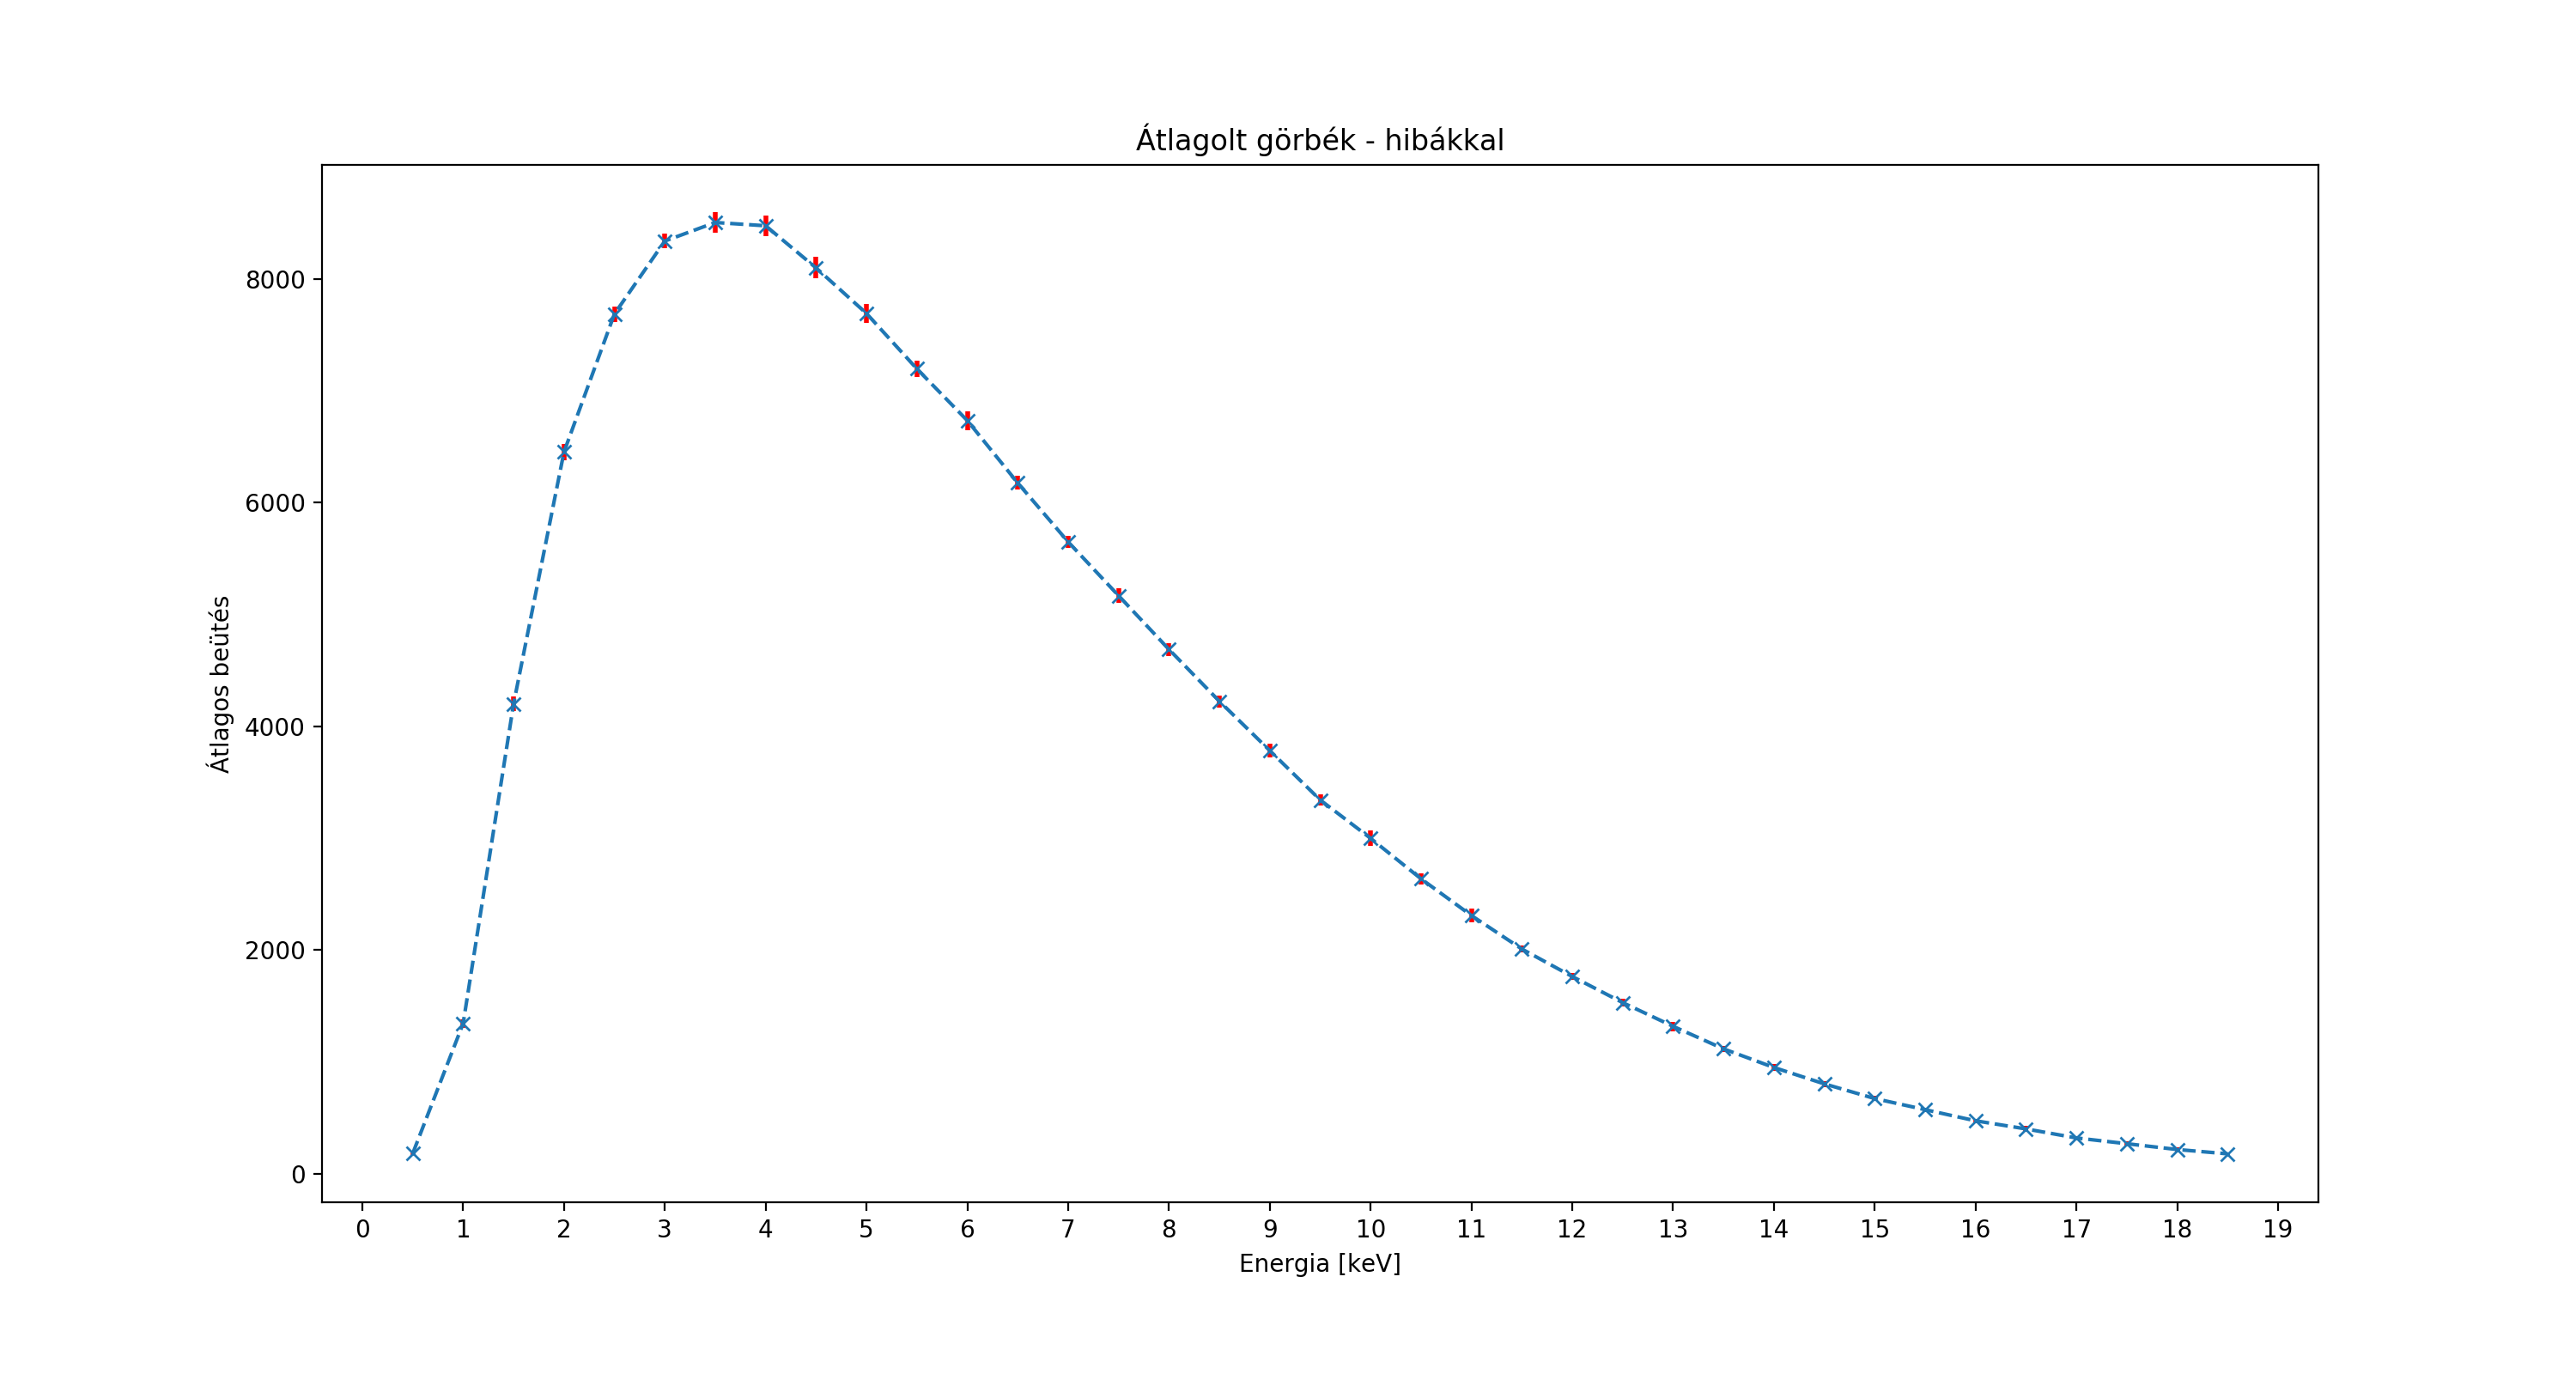
\includegraphics[width=0.9\linewidth ]{./atlagolt-gorbek-hibakkal.png}
	\caption{A spektrumok átlaga}
\end{figure}

\vspace{0.2cm}

\par Jól látható, hogy a hibák elenyészően kicsik, a különböző mérések
nagyban fedésben vannak.

\vspace{0.2cm}

\subsection{Szórás és beütés szám}

\par Az egyes `bin`-ekben lévő beütések hibáját ($\sigma$) véve
az átlag beütések számának a következő összefüggést kell elméleti
úton mutatnia:

\vspace{0.2cm}

\begin{equation*}
	\sigma^{2} = m\cdot N
\end{equation*}

\vspace{0.2cm}

\par Ahol N a beütések átlagos száma adott `bin`-ben, míg $\sigma$
a szórás.

\vspace{0.2cm}

\begin{figure}[H]
	\centering
	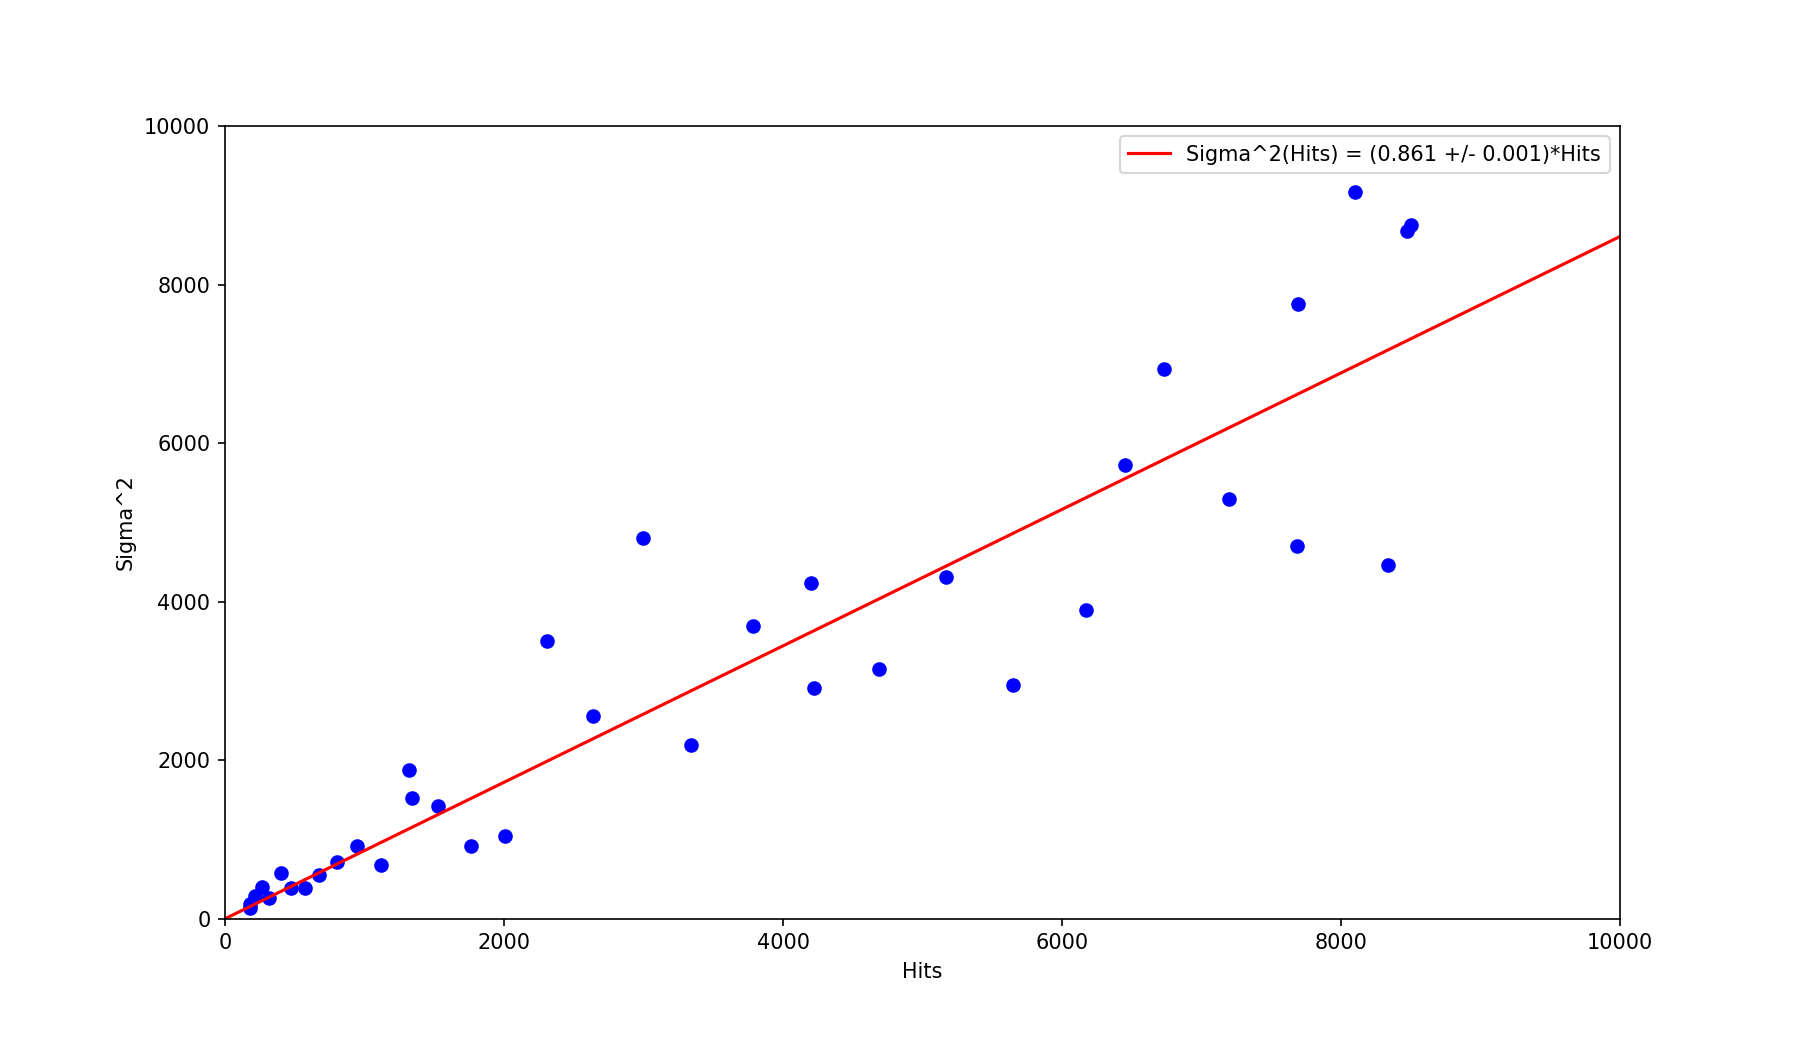
\includegraphics[width=0.75\linewidth ]{./szoras.png}
	\caption{Szórás}
\end{figure}

\vspace{0.2cm}

\par Látható, hogy az illesztés paraméterei:

\vspace{0.2cm}

\begin{equation*}
	\sigma^{2} = m*N = (0.861 \pm 0.001)*N
\end{equation*}

\vspace{0.2cm}

\subsection{Átlagos energia}

\par Az energia átlagok a súlyozott spektrum átlagokból pedig:

\vspace{0.2cm}

\begin{equation*}
	\big<E\big> = 6.1875 \pm 0.0076 ~keV
\end{equation*}

\vspace{0.2cm}

\par ami nagyban összevág a kívánt, elméleti adattal.

\vspace{0.2cm}

\begin{figure}[H]
	\centering
	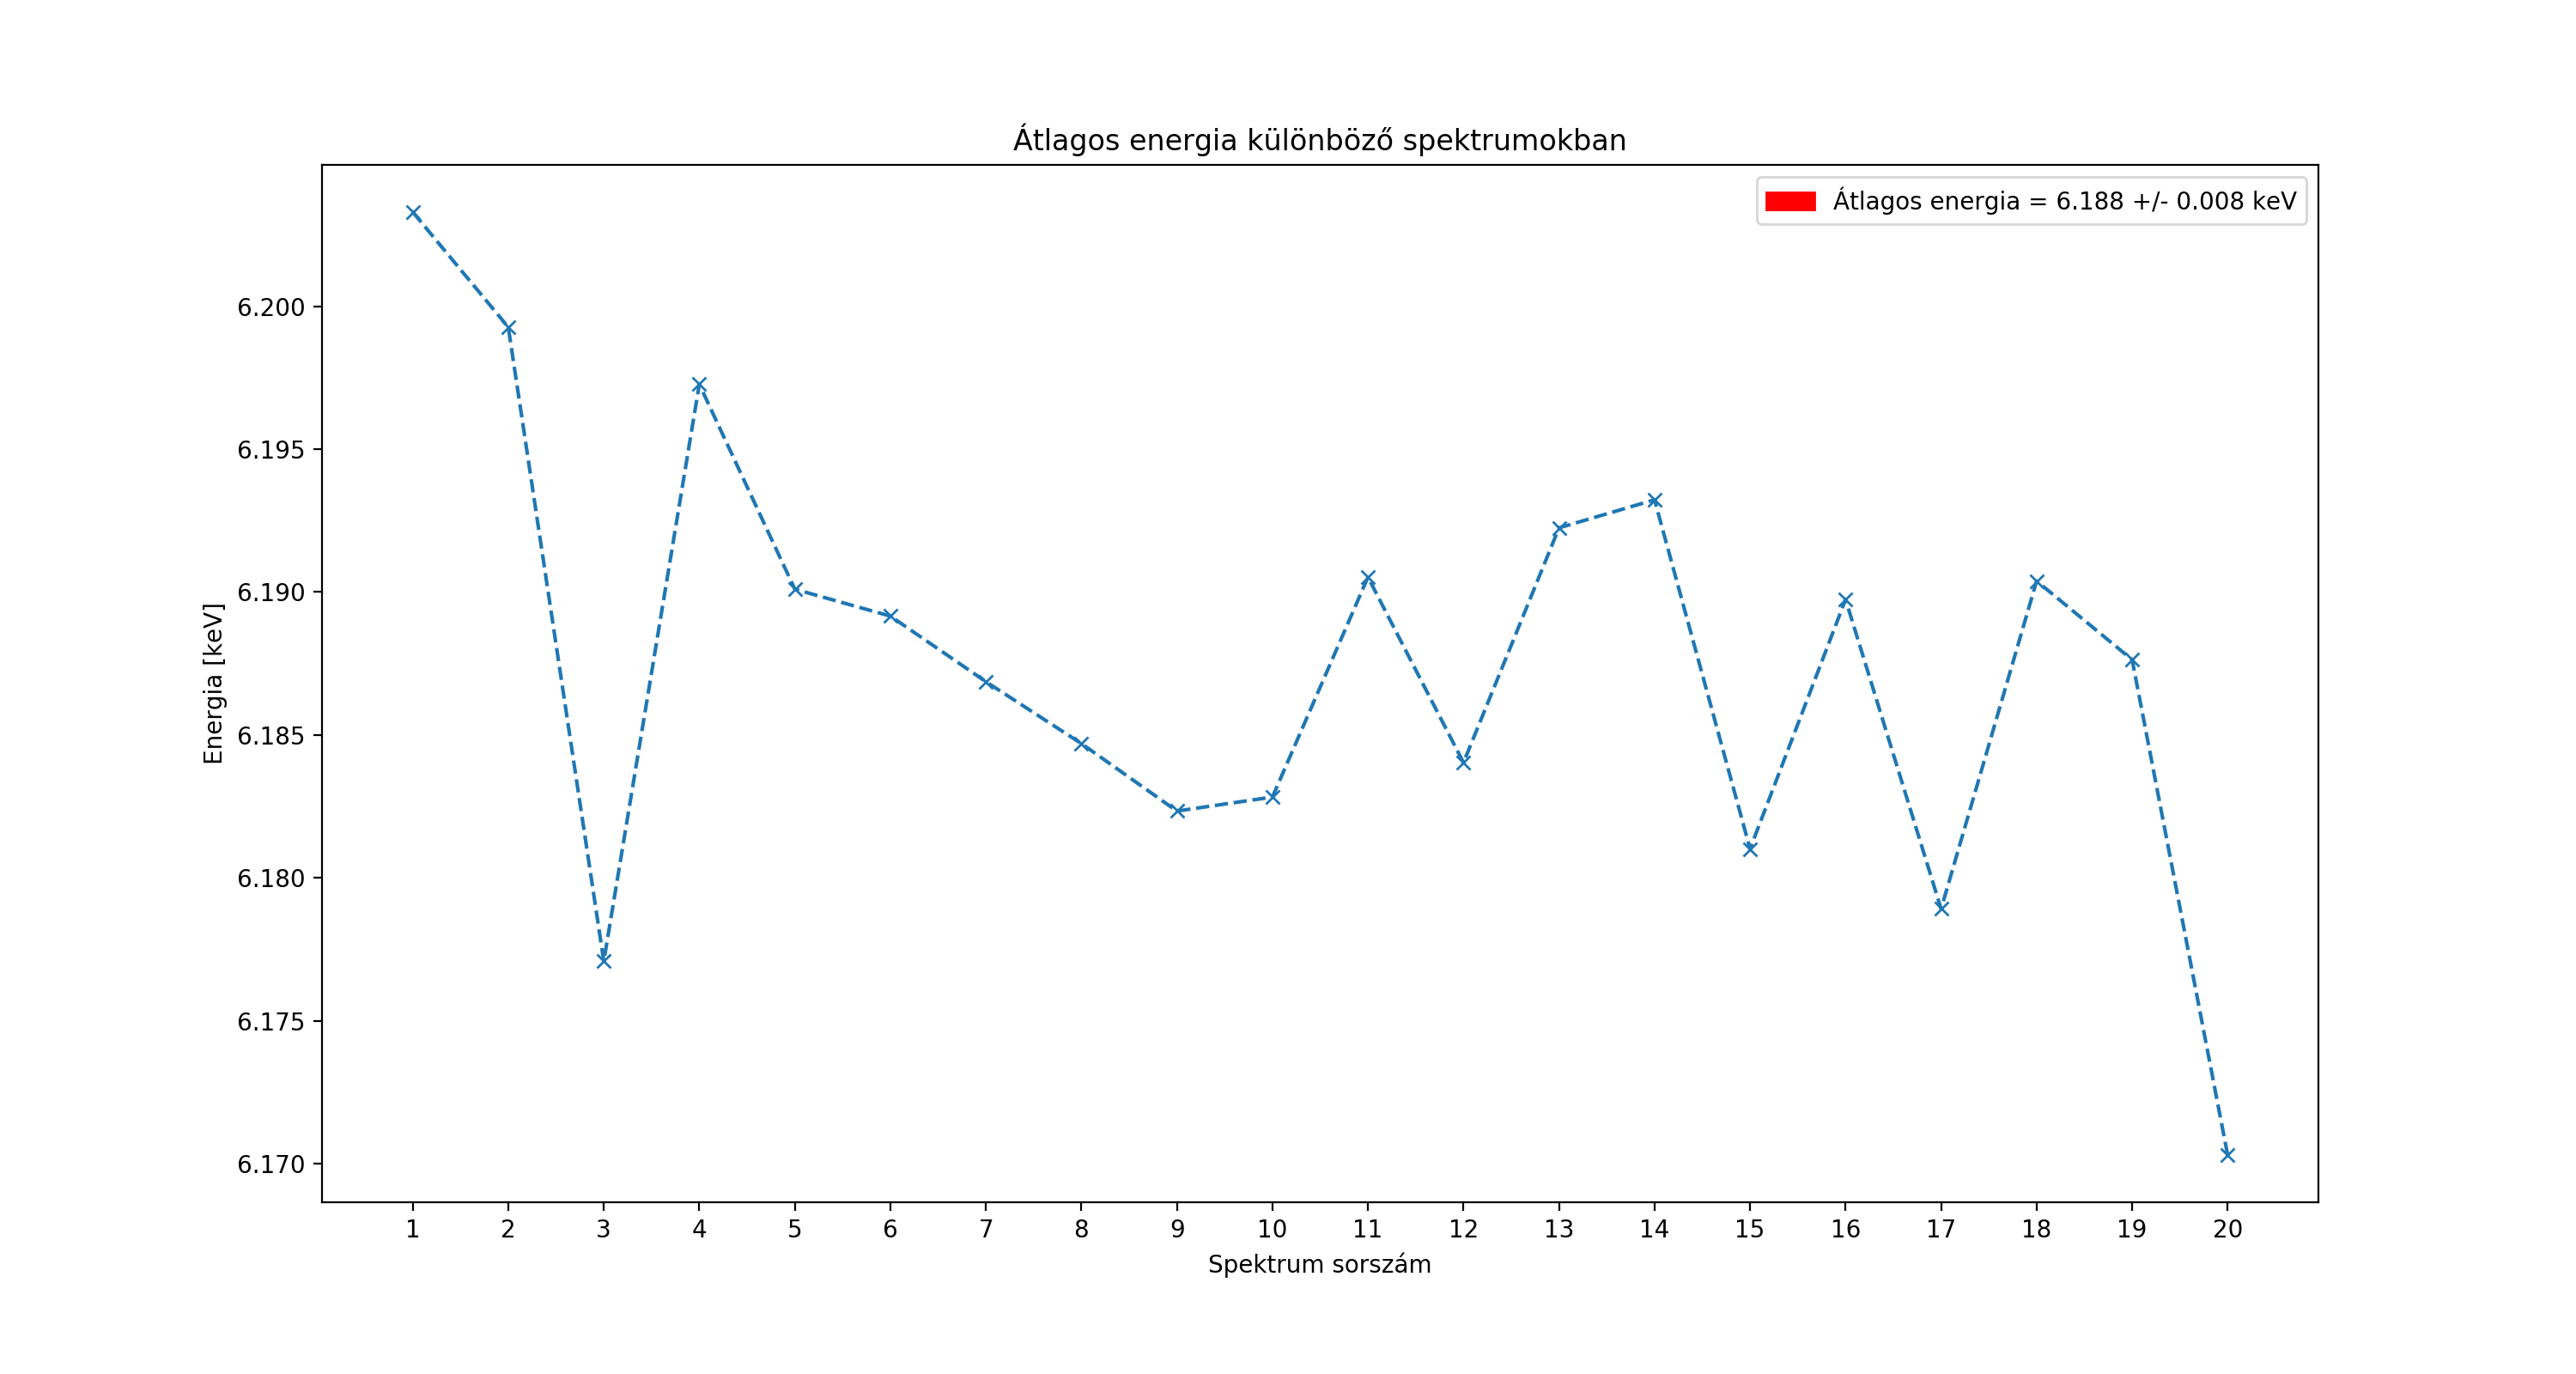
\includegraphics[width=0.8\linewidth ]{./atlagos-energia.png}
	\caption{Átlagos energia alakulása a különböző spektrumokban}
\end{figure}

\vspace{0.2cm}

\subsection{Illesztések}

\subsubsection{Fermi függvény nélkül}

\par Először az (1) - es összefüggést illesztettük meg. Ez többé kevésbé sikerült.
Az illesztés során két paramétert használtunk $Q$-t és egy normálási tényezőt
$N$-t. Az illesztést Pythonban végeztük el, és hiába állítottuk a paramétereket,
nem kaptunk sokkalta változatosabb illesztéseket. Az illesztett görbék
paramétereit táblázatban tüntetem fel és csak egy ábrát közlök, hiszen
feleslgeesnek érzem mind a 19-et belerakni a jegyzőkönyvbe.

\vspace{0.2cm}

\begin{table}[H]
	\centering
	\begin{tabular}{|c|c|} \hline
		Norm factor          & Q [keV]            \\ \hline
		0.0001 $\pm$ 0.00000 & 17.662 $\pm$ 0.544 \\ \hline
		0.0001 $\pm$ 0.00000 & 17.645 $\pm$ 0.553 \\ \hline
		0.0001 $\pm$ 0.00000 & 17.588 $\pm$ 0.532 \\ \hline
		0.0001 $\pm$ 0.00000 & 17.628 $\pm$ 0.542 \\ \hline
		0.0001 $\pm$ 0.00000 & 17.633 $\pm$ 0.546 \\ \hline
		0.0001 $\pm$ 0.00000 & 17.598 $\pm$ 0.545 \\ \hline
		0.0001 $\pm$ 0.00000 & 17.595 $\pm$ 0.552 \\ \hline
		0.0001 $\pm$ 0.00000 & 17.589 $\pm$ 0.530 \\ \hline
		0.0001 $\pm$ 0.00000 & 17.580 $\pm$ 0.548 \\ \hline
		0.0001 $\pm$ 0.00000 & 17.596 $\pm$ 0.557 \\ \hline
		0.0001 $\pm$ 0.00000 & 17.601 $\pm$ 0.536 \\ \hline
		0.0001 $\pm$ 0.00000 & 17.592 $\pm$ 0.544 \\ \hline
		0.0001 $\pm$ 0.00000 & 17.638 $\pm$ 0.553 \\ \hline
		0.0001 $\pm$ 0.00000 & 17.625 $\pm$ 0.559 \\ \hline
		0.0001 $\pm$ 0.00000 & 17.606 $\pm$ 0.538 \\ \hline
		0.0001 $\pm$ 0.00000 & 17.612 $\pm$ 0.551 \\ \hline
		0.0001 $\pm$ 0.00000 & 17.561 $\pm$ 0.553 \\ \hline
		0.0001 $\pm$ 0.00000 & 17.621 $\pm$ 0.550 \\ \hline
		0.0001 $\pm$ 0.00000 & 17.612 $\pm$ 0.550 \\ \hline
		0.0001 $\pm$ 0.00000 & 17.544 $\pm$ 0.550 \\ \hline
	\end{tabular}
\end{table}

\vspace{0.2cm}

\begin{figure}[H]
	\centering
	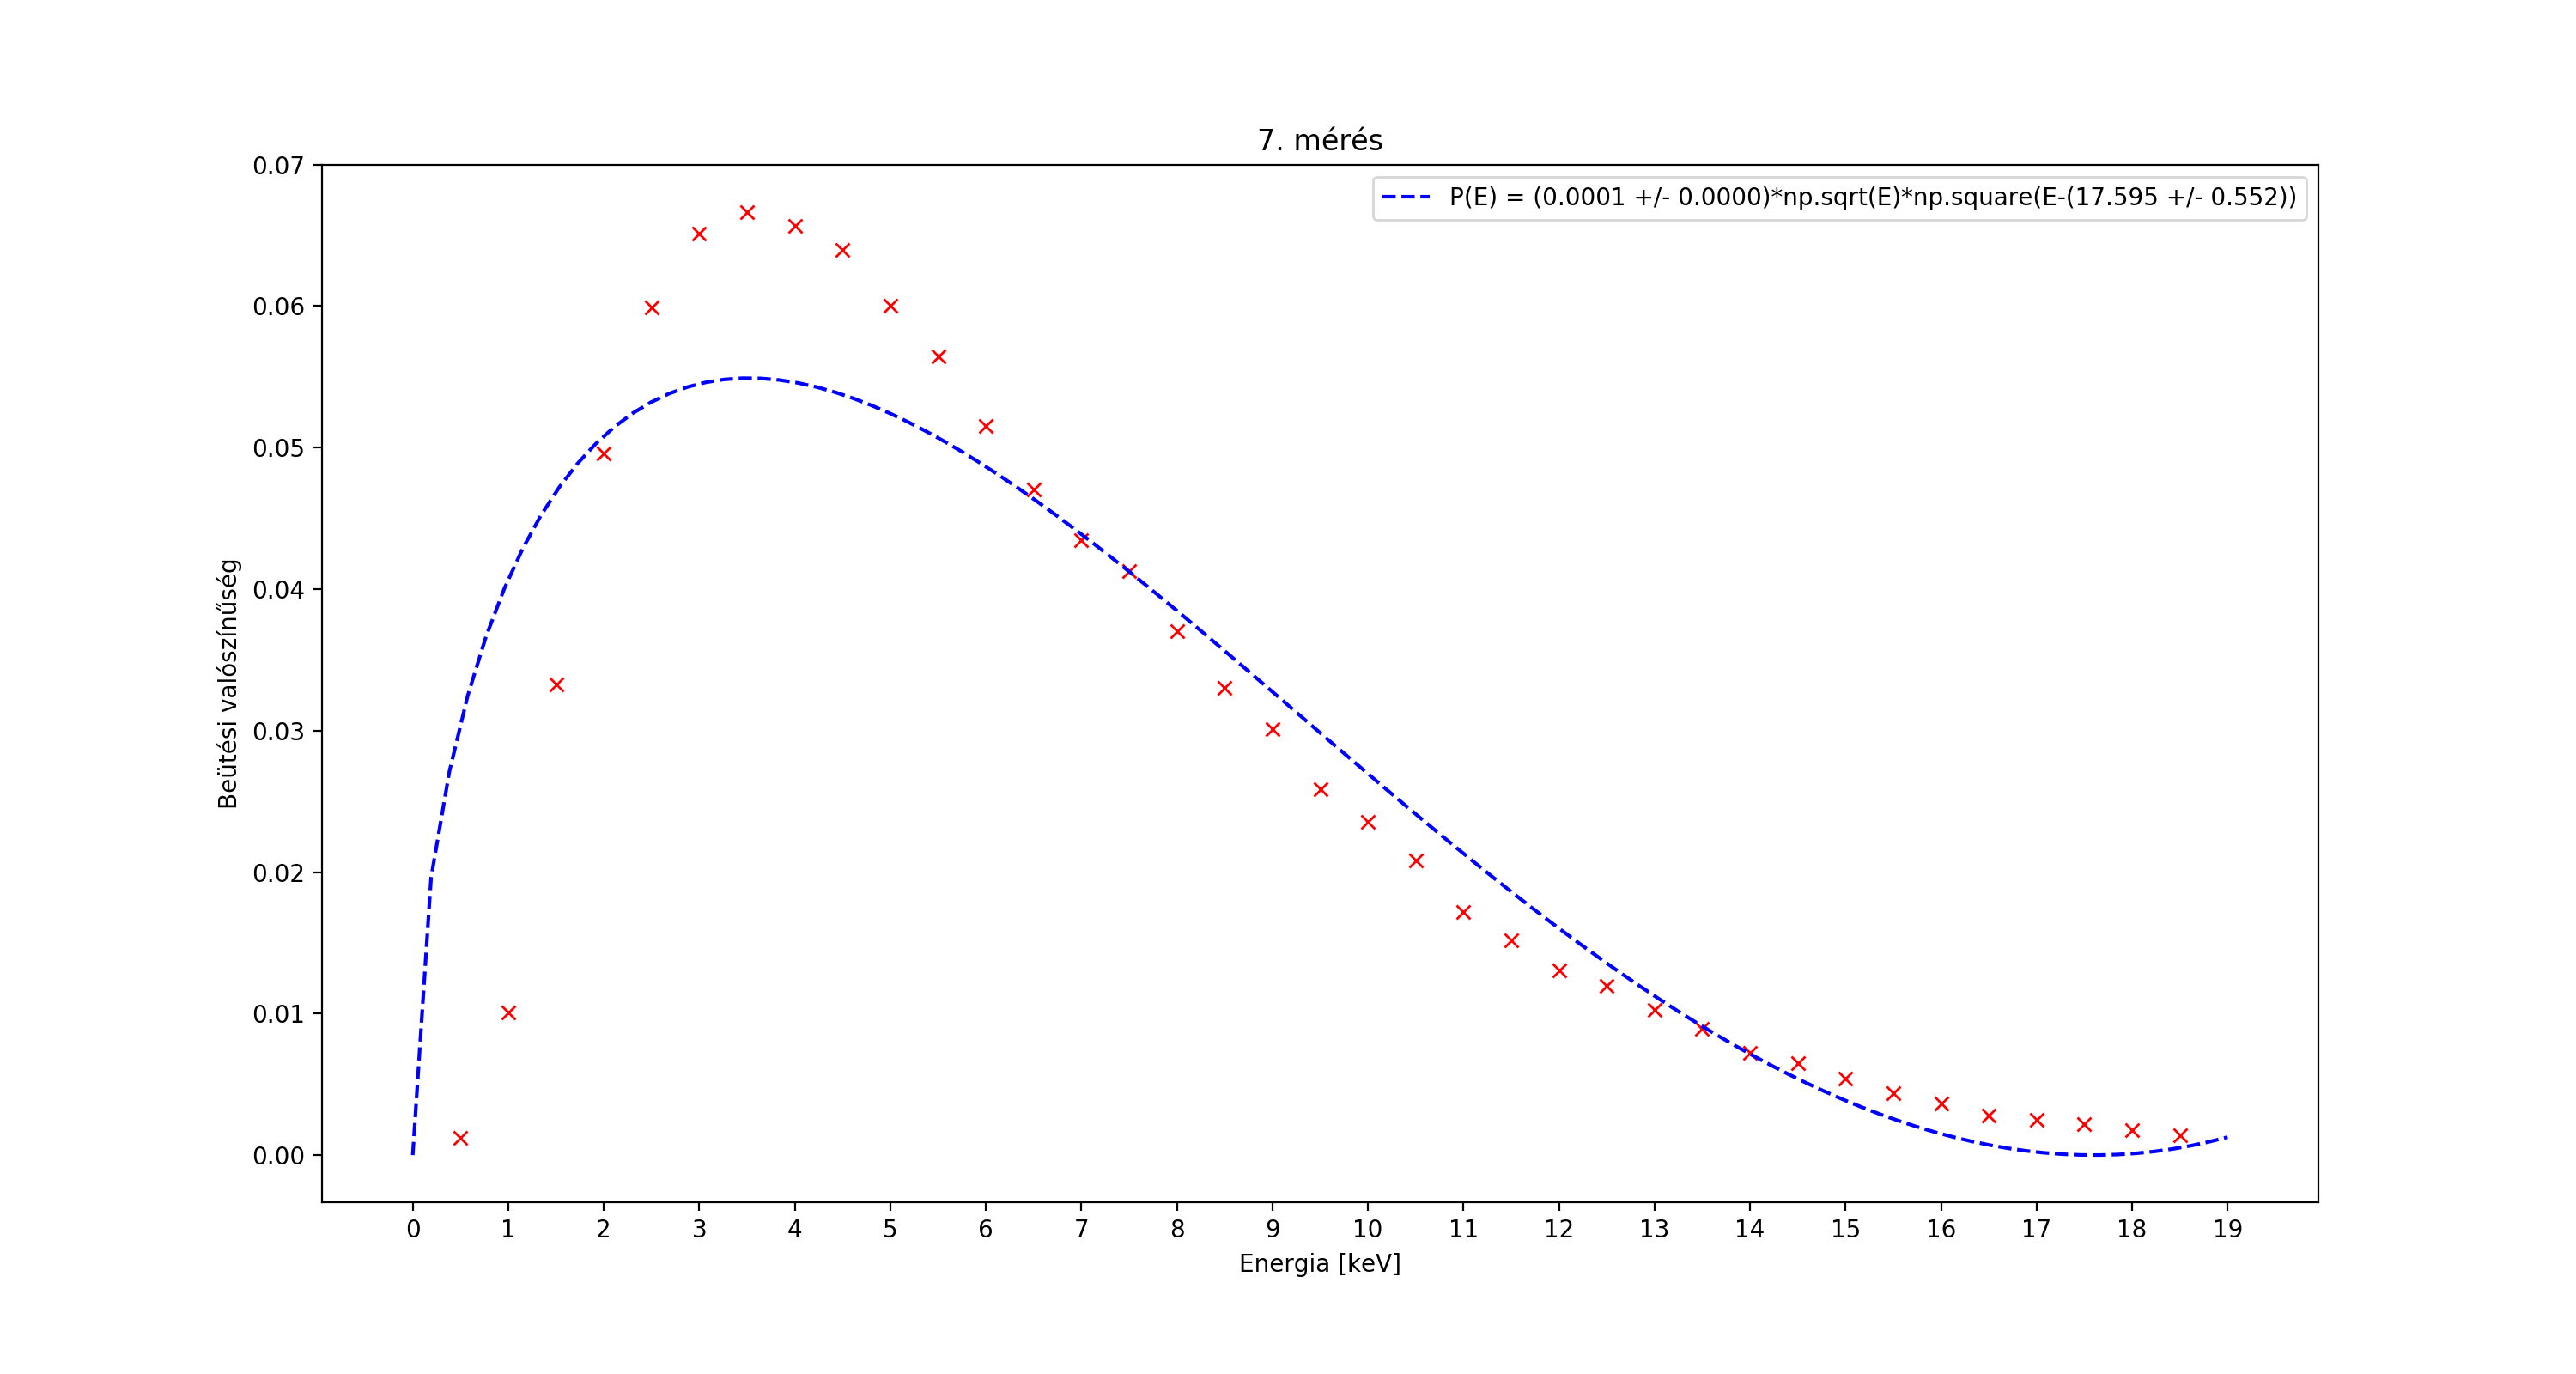
\includegraphics[width=0.95\linewidth ]{./atlagolt-gorbek-hibakkal6.png}
	\caption{A 7. illesztés - paraméterivel}
\end{figure}

\vspace{0.2cm}

\subsubsection{Fermi fügvénnyel}

\par Az irodalomban [2] található Fermi-függvényt használva, mely
kisebb magokra, $\beta^{-}$-bomlásra a következő:

\vspace{0.2cm}

\begin{align*}
	P(E)_{\eta} = \eta^{2}P(E)2\pi \frac{Y(\eta)}{(1-e^{-2\pi Y(\eta)})} \\
	P(E) = N\sqrt{E}(E - Q)^{2}                                          \\
	Y(\eta) =  \frac{3}{137}\cdot\frac{(1 + \eta^{2})^{\frac{1}{2}}}{\eta}
\end{align*}

\vspace{0.2cm}

\par Jól láható, hogy $P(E)_{\eta}$ egy három paraméteres függvény
melynek illesztése nem triviális és a számítógép nem is bírkózott meg vele
sajnálatos módon. Ezért azt a módszert alkalmaztuk, hogy a felhasználtuk
az előző illesztés $N, Q$  paramétereit és csakis az $\eta$
paramétert illesztettük meg az előbbi függvényben. Ezáltal az illesztések
konvergáltak, de precízek sajnos nem lettek.

\vspace{0.2cm}

\vspace{0.2cm}

\begin{table}[H]
	\centering
	\begin{tabular}{|c|c|c|} \hline
		$\eta$              & Norm factor          & Q [keV]            \\ \hline
		0.9521 $\pm$ 0.0004 & 0.0001 $\pm$ 0.00000 & 17.662 $\pm$ 0.544 \\ \hline
		0.9521 $\pm$ 0.0004 & 0.0001 $\pm$ 0.00000 & 17.645 $\pm$ 0.553 \\ \hline
		0.9521 $\pm$ 0.0004 & 0.0001 $\pm$ 0.00000 & 17.588 $\pm$ 0.532 \\ \hline
		0.9521 $\pm$ 0.0004 & 0.0001 $\pm$ 0.00000 & 17.628 $\pm$ 0.542 \\ \hline
		0.9521 $\pm$ 0.0004 & 0.0001 $\pm$ 0.00000 & 17.633 $\pm$ 0.546 \\ \hline
		0.9521 $\pm$ 0.0004 & 0.0001 $\pm$ 0.00000 & 17.598 $\pm$ 0.545 \\ \hline
		0.9521 $\pm$ 0.0004 & 0.0001 $\pm$ 0.00000 & 17.595 $\pm$ 0.552 \\ \hline
		0.9521 $\pm$ 0.0004 & 0.0001 $\pm$ 0.00000 & 17.589 $\pm$ 0.530 \\ \hline
		0.9521 $\pm$ 0.0004 & 0.0001 $\pm$ 0.00000 & 17.580 $\pm$ 0.548 \\ \hline
		0.9521 $\pm$ 0.0004 & 0.0001 $\pm$ 0.00000 & 17.596 $\pm$ 0.557 \\ \hline
		0.9521 $\pm$ 0.0004 & 0.0001 $\pm$ 0.00000 & 17.601 $\pm$ 0.536 \\ \hline
		0.9521 $\pm$ 0.0004 & 0.0001 $\pm$ 0.00000 & 17.592 $\pm$ 0.544 \\ \hline
		0.9521 $\pm$ 0.0004 & 0.0001 $\pm$ 0.00000 & 17.638 $\pm$ 0.553 \\ \hline
		0.9521 $\pm$ 0.0004 & 0.0001 $\pm$ 0.00000 & 17.625 $\pm$ 0.559 \\ \hline
		0.9521 $\pm$ 0.0004 & 0.0001 $\pm$ 0.00000 & 17.606 $\pm$ 0.538 \\ \hline
		0.9521 $\pm$ 0.0004 & 0.0001 $\pm$ 0.00000 & 17.612 $\pm$ 0.551 \\ \hline
		0.9521 $\pm$ 0.0004 & 0.0001 $\pm$ 0.00000 & 17.561 $\pm$ 0.553 \\ \hline
		0.9521 $\pm$ 0.0004 & 0.0001 $\pm$ 0.00000 & 17.621 $\pm$ 0.550 \\ \hline
		0.9521 $\pm$ 0.0004 & 0.0001 $\pm$ 0.00000 & 17.612 $\pm$ 0.550 \\ \hline
		0.9521 $\pm$ 0.0004 & 0.0001 $\pm$ 0.00000 & 17.544 $\pm$ 0.550 \\ \hline
	\end{tabular}
\end{table}

\par $\eta$ lényegében konstans lett minden egyes görbére. Ez nem feltétlenül probléma
abból a szempontból, hogy a görbék, mint az az átlagolás során kiderült nem térnek
el jelentős mértékben. Itt is egy ábrát mellékelek csak.

\begin{figure}[H]
	\centering
	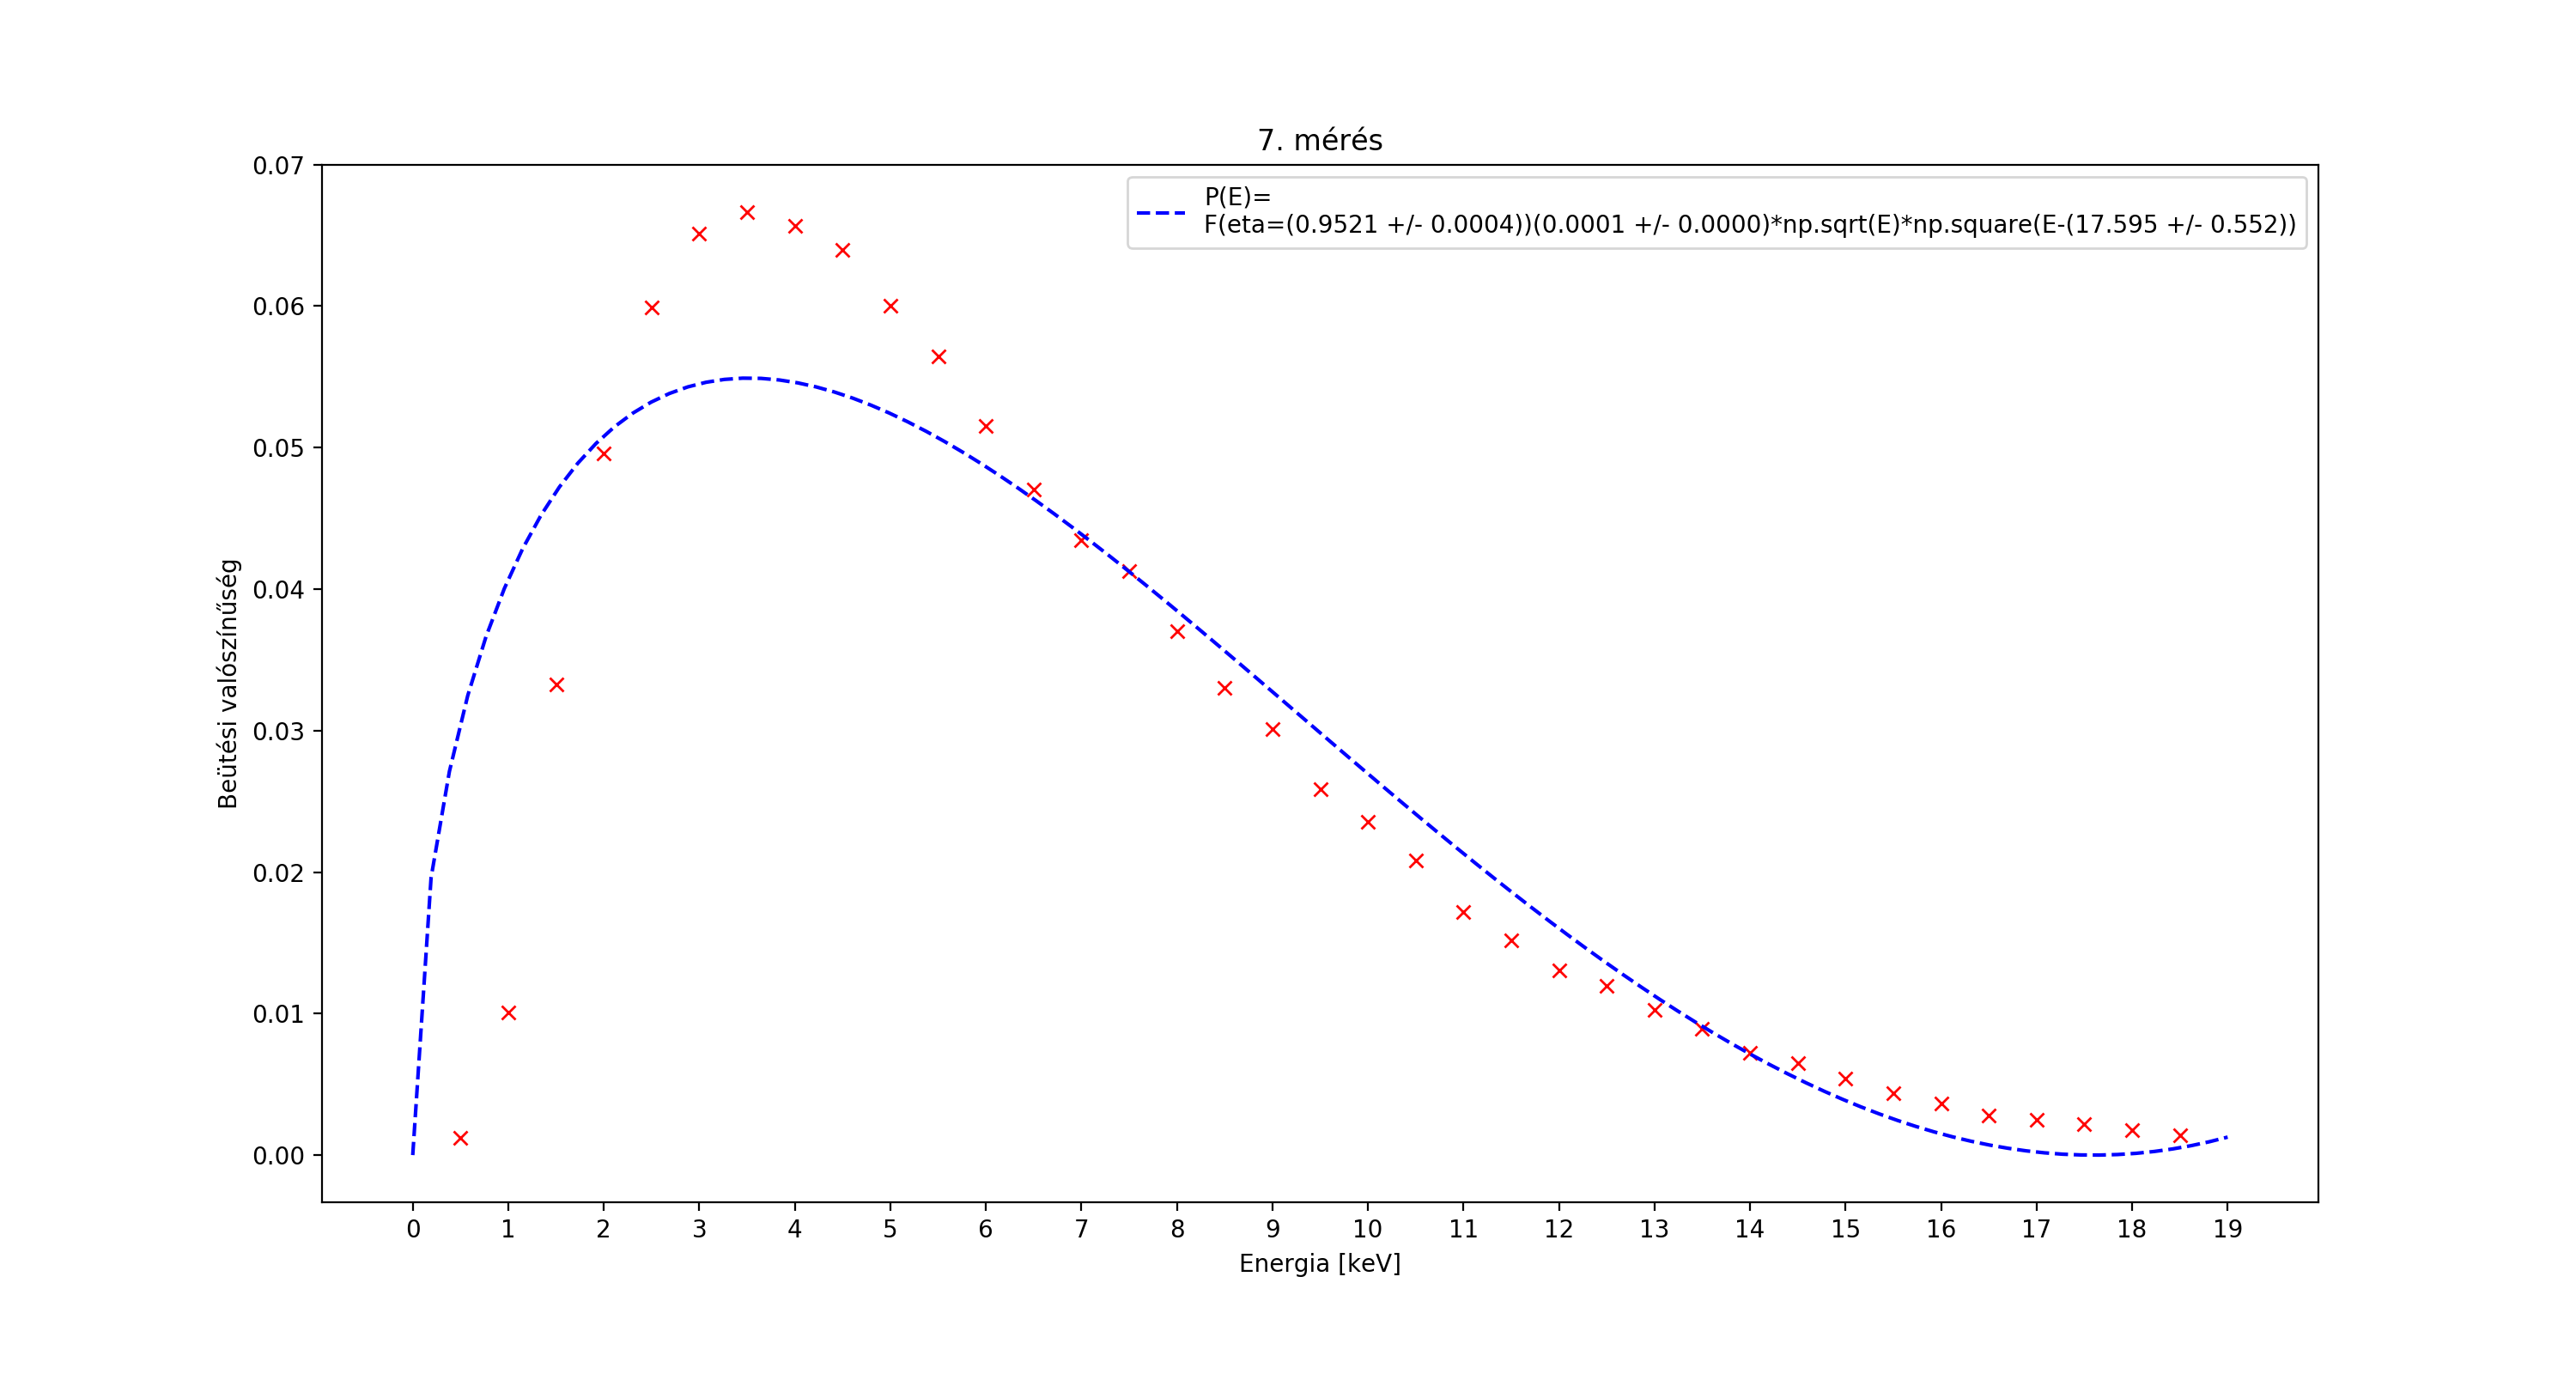
\includegraphics[width=0.95\linewidth ]{./atlagolt-gorbek-hibakkal-fermi6.png}
	\caption{A 7. illesztés - paraméterivel}
\end{figure}

\section{Diszkusszió}
\hspace*{10pt} A mérés során a műszerhez kapcsolt számítógép kék halált kapott.
A gép csatlakoztatva van az internetre és még mindig csak Windows XP fut rajta.
A mérési adatokat ezért később kaptuk meg és a mérést nem mi végeztük el valójában.

\newpage

\section*{Hivatkozások}
\begin{itemize}
	\item[[1]] {http://metal.elte.hu/oktatas/alkfizlab/meresleirasok/FSS.pdf}
	\item[[2]] {I. Feister - Numerical evaluation of the Fermi-Beta Distribution Function}

\end{itemize}
\end{document}
\end{document}